\section*{Aufgabe 4 (25 Punkte)}
\vspace{0.4cm}
\subsection*{\frage{1}{3}}
Das bestimmte Integral
\begin{align*}
\int_0^\pi 2 \ \sin(x) \ \cos(x) \ dx
\end{align*}
hat den Wert
\renewcommand{\labelenumi}{(\alph{enumi})}
\begin{enumerate}
	\item 
	$0$.
	\item
	$1$.
	\item
	$2$.
	\item
	Keines der obigen Resultate ist korrekt.
\end{enumerate}
\ \\
\textbf{Lösung:}
\begin{mdframed}
\underline{\textbf{Vorgehensweise:}}
\renewcommand{\labelenumi}{\theenumi.}
\begin{enumerate}
\item Forme den Integranden um und finde die korrekte Antwort.
\end{enumerate}
\end{mdframed}

\underline{1. Forme den Integranden um und finde die korrekte Antwort}\\
Das Additionstheorem der Sinusfunktion besagt
\begin{align*}
\sin(x + y)
= \sin(x) \cdot \cos(y) + \cos(x) \cdot \sin(y).
\end{align*}
Mit $ x = y  $ erhalten wir den Integranden:
\begin{align*}
\sin(2x) = 2 \sin(x) \cos(x).
\end{align*}
Der Term $ \sin(2x) $ ist auf dem Intervall $ [0,\pi] $ punktsymmetrisch in der Achse $ \frac{\pi}{2} $.
Dementsprechend folgt
\begin{align*}
\int_0^\pi 2 \ \sin(x) \ \cos(x) \ dx
=
\int_0^\pi \sin(2x) \ dx = 0.
\end{align*}
\begin{center}
	\begin{tikzpicture}
	\begin{axis}[
	domain=0:3.1416,
	xmin=0, xmax=3.1416,
	ymin=-1.1, ymax=1.1,
	samples=400,
	axis y line=center,
	axis x line=middle,
	]
	\addplot+[mark=none] { sin(deg(2*x)};
	%\addplot+[mark=none] { sin(deg(2*x)};
	\legend{$ \sin(2x) $}
	\end{axis}
	\end{tikzpicture}
\end{center}

Die Aufgabe lässt sich auch durch Substitution lösen.
Mit $ t = \sin(x) $ erhalten wir wegen $ \frac{dt}{dx} = \cos(x)  $ das Resultat
\begin{align*}
\int_0^\pi 2 \ \sin(x) \ \cos(x) \ dx
=
\int_0^0 2 t \ dt = 0.
\end{align*}
Wichtig ist hierbei, dass die Grenzen mit substituiert wurden.\\
\\
Damit ist Antwort (a) korrekt.\\
\\
\textit{
Da $ \sin(x) $ achsensymmetrisch und $ \cos(x) $ punktsymmetrisch auf dem Intervall $ [0,\pi] $ in der Achse $ \frac{\pi}{2} $ ist, ist deren Produkt auch punktsymmetrisch in der Achse $ \frac{\pi }{2} \approx 1.571 $.\\
\\
\begin{center}
	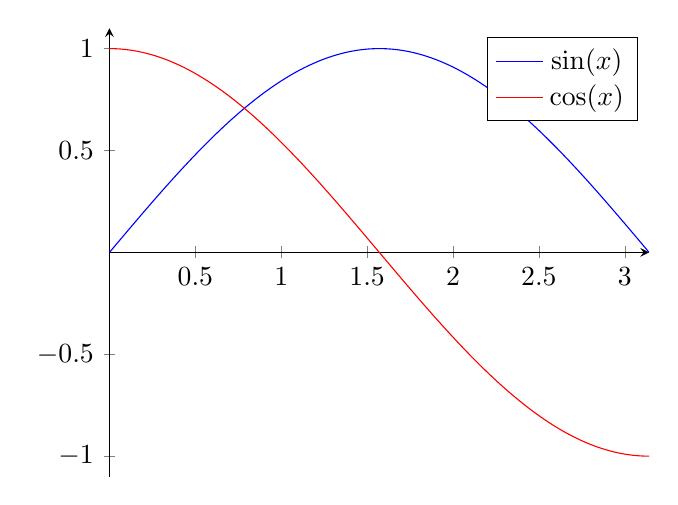
\begin{tikzpicture}
	\begin{axis}[
	domain=0:3.1416,
	xmin=0, xmax=3.1416,
	ymin=-1.1, ymax=1.1,
	samples=400,
	axis y line=center,
	axis x line=middle,
	]
	\addplot+[mark=none] { sin(deg(x)};
	\addplot+[mark=none] { cos(deg(x)};
	\legend{$ \sin(x) $,$ \cos(x) $}
	\end{axis}
	\end{tikzpicture}
\end{center}
Damit folgt auch direkt, dass (a) die korrekte Antwort ist.
}



\newpage

\subsection*{\frage{2}{3}}
Für welchen Wert von $ t \in \mathbb{R} $ sind die Vektoren $ \textbf{u} = \begin{pmatrix}
t-2 \\ t \\ 3
\end{pmatrix} $ und $ \textbf{v} = \begin{pmatrix}
1 \\ t-1 \\ 9
\end{pmatrix} $ orthogonal?
\renewcommand{\labelenumi}{(\alph{enumi})}
\begin{enumerate}
\item 
$t = 5$.
\item
$t = 5$ oder $ t = -5 $.
\item
$ \textbf{u} $ und $ \textbf{v}  $ sind für kein $ t \in \mathbb{R} $ orthogonal.
\item
$ \textbf{u} $ und $ \textbf{v}  $ sind für alle $ t \in \mathbb{R} $ orthogonal.
\end{enumerate}
\ \\
\textbf{Lösung:}
\begin{mdframed}
\underline{\textbf{Vorgehensweise:}}
\renewcommand{\labelenumi}{\theenumi.}
\begin{enumerate}
\item Berechne das Skalarprodukt der Vektoren.
\end{enumerate}
\end{mdframed}

\underline{1. Berechne das Skalarprodukt der Vektoren}\\
Das Skalarprodukt liefert
\begin{align*}
\textbf{u} \cdot \textbf{v}
=
\begin{pmatrix}
t-2 \\ t \\ 3
\end{pmatrix}
\cdot 
\begin{pmatrix}
1 \\ t-1 \\ 9
\end{pmatrix}
=
(t-2) \cdot 1 + t ( t-1) + 3 \cdot 9
=
t-2 + t^2 -t + 27
=t^2 + 25.
\end{align*}
Die Vektoren $ \textbf{u} $ und $ \textbf{v} $ sind genau dann orthogonal, falls
\begin{align*}
\textbf{u} \cdot \textbf{v} = t^2 + 25 = 0
\ \Leftrightarrow \
t^2 = -25
\end{align*}
gilt. Nun ist $ t^2 = -25 $ für kein $ t \in \mathbb{R} $ erfüllt.\\
\\
Damit ist Antwort (c) korrekt.
\newpage
\subsection*{\frage{3}{4}}
Die $4 \times 5$ Matrix
\begin{align*}
A
=
\begin{pmatrix}
1 & 1  & 3 & -1 & -2 \\
3 & -5  & -7 & 13 & -10 \\
-1 & 3  & 5 & -7 & 4 \\
-2 & 10  & 18 & -22 & 10  
\end{pmatrix}
\end{align*}
\renewcommand{\labelenumi}{(\alph{enumi})}
\begin{enumerate}
	\item 
	hat Rang $2$.
	\item
	hat Rang $3$.
	\item
	hat Rang $4$.
	\item
	hat Rang $5$.
\end{enumerate}
\ \\
\textbf{Lösung:}
\begin{mdframed}
\underline{\textbf{Vorgehensweise:}}
\renewcommand{\labelenumi}{\theenumi.}
\begin{enumerate}
\item Wende das Gauß-Verfahren an.
\item Bestimme den Rang mithilfe der Nullzeilen.
\end{enumerate}
\end{mdframed}
%\allowdisplaybreaks
\underline{1. Wende das Gauß-Verfahren an}\\
Das Gauß-Verfahren liefert:
\begin{align*}
A=
\begin{gmatrix}[p]
1 & 1  & 3 & -1 & -2 \\
3 & -5  & -7 & 13 & -10 \\
-1 & 3  & 5 & -7 & 4 \\
-2 & 10  & 18 & -22 & 10  
\rowops
\add[-3]{0}{1}
\add[1]{0}{2}
\add[2]{0}{3}
\end{gmatrix}
&\leadsto
\begin{gmatrix}[p]
1 & 1  & 3 & -1 & -2 \\
0 & -8  & -16 & 16 & -4 \\
0 & 4  & 8 & -8 & 2 \\
0 & 12  & 24 & -24 & 6  
\rowops
\mult{1}{\cdot ( -\frac{1}{4} )}
\mult{2}{\cdot ( \frac{1}{2} )}
\mult{3}{\cdot ( \frac{1}{6} )}
\end{gmatrix}\\
&\leadsto
\begin{gmatrix}[p]
1 & 1  & 3 & -1 & -2 \\
0 & 2  & 4 & -4 & 1 \\
0 & 2  & 4 & -4 & 1 \\
0 & 2  & 4 & -4 & 1 
\rowops
\add[-1]{1}{2}
\add[-1]{1}{3}
\end{gmatrix}\\
&\leadsto
\begin{gmatrix}[p]
1 & 1  & 3 & -1 & -2 \\
0 & 2  & 4 & -4 & 1 \\
0 & 0  & 0 & 0 & 0 \\
0 & 0  & 0 & 0 & 0 
\end{gmatrix}
= A^\star.
\end{align*}
\ \\
\underline{2. Bestimme den Rang mithilfe der Nullzeilen}\\
Die Matrix hat zwei Nullzeilen.
Folglich gilt $ \text{rg}(A) = \text{rg}(A^\star) = 4 - 2 = 2 $.\\
\\
%Wegen $ \text{rg}(A) = \text{rg}(A^\star) $ und $ \text{rg}(A^\star) = 2 $ ist Antwort (a) korrekt.
Damit ist Antwort (a) korrekt.
\newpage
\subsection*{\frage{4}{4}}
Gesucht ist eine Matrix $ X $, sodass
\begin{align*}
X
\begin{pmatrix}
1 & 2 \\
0 & 1 
\end{pmatrix}
=
\begin{pmatrix}
4 & 3 \\
2 & 1
\end{pmatrix}
.
\end{align*}
\renewcommand{\labelenumi}{(\alph{enumi})}
\begin{enumerate}
	\item 
	$X
	= 
	\begin{pmatrix}
	1 & 3  \\
	-2 & -1 
	\end{pmatrix}$.
	\item
	$X
	= 
	\begin{pmatrix}
	4 &-5  \\
	2 & -3 
	\end{pmatrix}$.
	\item
	$X
	= 
	\begin{pmatrix}
	4 &-3  \\
	-2 & 4 
	\end{pmatrix}$.
	\item
	Es gibt keine Matrix $ X $, die die Gleichung erfüllt.
\end{enumerate}
\ \\
\textbf{Lösung:}
\begin{mdframed}
\underline{\textbf{Vorgehensweise:}}
\renewcommand{\labelenumi}{\theenumi.}
\begin{enumerate}
\item Finde die Lösung durch invertieren einer Matrix.

\end{enumerate}
\end{mdframed}

\underline{1. Finde die Lösung durch das Invertieren einer Matrix}\\
Zunächst betrachten wir die Gleichung
\begin{align*}
X
\begin{pmatrix}
1 & 2 \\
0 & 1 
\end{pmatrix}
=
\begin{pmatrix}
4 & 3 \\
2 & 1
\end{pmatrix}
.
\end{align*}
Die bekannte Matrix ist invertierbar, da
\begin{align*}
\det \begin{pmatrix}
1 & 2 \\
0 & 1 
\end{pmatrix}
= 1 \cdot 1 - 0 \cdot 2 = 1 \neq 0
\end{align*}
gilt.
Für die Inverse einer $ 2 \times 2 $  Matrix gilt:
\begin{align*}
\begin{pmatrix}
a & b \\
c & d
\end{pmatrix}^{-1}
= 
\frac{1}{\det \begin{pmatrix}
	a & b \\
	c & d
	\end{pmatrix}}
\begin{pmatrix}
d & -b \\
-c & a
\end{pmatrix}
= \frac{1}{a d - bc} 
\begin{pmatrix}
d & -b \\
-c & a
\end{pmatrix}.
\end{align*}
Damit erhalten wir 
\begin{align*}
\begin{pmatrix}
1 & 2 \\
0 & 1 
\end{pmatrix}^{-1}
=
\frac{1}{1 \cdot 1 - 2 \cdot 0}
\begin{pmatrix}
1 & -2 \\
0 & 1 
\end{pmatrix}
= \begin{pmatrix}
1 & -2\\
0 & 1
\end{pmatrix}
\end{align*}
und es folgt:
\begin{align*}
X
\begin{pmatrix}
1 & 2 \\
0 & 1 
\end{pmatrix}
=
\begin{pmatrix}
4 & 3 \\
2 & 1
\end{pmatrix}
\Leftrightarrow
X
&=
\begin{pmatrix}
4 & 3 \\
2 & 1
\end{pmatrix}
\begin{pmatrix}
1 & 2 \\
0 & 1 
\end{pmatrix}^{-1}
= 
\begin{pmatrix}
4 & 3 \\
2 & 1
\end{pmatrix}
\begin{pmatrix}
1 & -2 \\
0 & 1 
\end{pmatrix}\\
&=
\begin{pmatrix}
4 \cdot 1+ 3\cdot 0 & 4 \cdot(-2) + 3 \cdot 1 \\
2 \cdot 1 + 1 \cdot 0 & 2 \cdot(-2) + 1 \cdot 1 
\end{pmatrix}
=
\begin{pmatrix}
4 & -5\\
2 & -3
\end{pmatrix}
\end{align*}
\ \\
Damit ist Antwort (b) korrekt.\\
\\
\textit{
Da hier $ 2 \times 2 $ Matrizen gegeben sind, bietet es sich auch an, die Möglichkeiten einzusetzen und nachzurechnen.
}

\newpage

\subsection*{\frage{5}{2}}
Die $ n \times n $ Matrix habe die Eigenwerte $ \lambda_1, \lambda_2, \dots, \lambda_n $.
Dann hat die Matrix $ A^2 $
\renewcommand{\labelenumi}{(\alph{enumi})}
\begin{enumerate}
	\item 
	die gleichen Eigenwerte.
	\item
	die Eigenwerte $2 \lambda_1,2 \lambda_2, \dots,2 \lambda_n $.
	\item
	die Eigenwerte $ \lambda_1^2, \lambda_2^2, \dots, \lambda_n^2 $.
	\item
	Keine der vorangehenden Antworten ist richtig.
\end{enumerate}
\ \\
\textbf{Lösung:}
\begin{mdframed}
\underline{\textbf{Vorgehensweise:}}
\renewcommand{\labelenumi}{\theenumi.}
\begin{enumerate}
\item Rufe dir die Definition eines Eigenwertes in Erinnerung und löse damit die Aufgabe.
\end{enumerate}
\end{mdframed}

\underline{1. Rufe dir die Definition eines Eigenwertes in Erinnerung und löse damit die Aufgabe}\\
Sei $ A $ eine $ n \times n$ Matrix. Dann heißt  $ \textbf{v} \in \mathbb{R}^n $ Eigenvektor zu dem Eigenwert $ \lambda $, falls
\begin{align*}
A \textbf{v} = \lambda \textbf{v}
\end{align*}
gilt. Dementsprechend erhalten wir mit
\begin{align*}
A^2 \textbf{v} = \lambda  A \textbf{v} = \lambda \cdot \lambda   \textbf{v}= \lambda^2 \textbf{v}, 
\end{align*}
dass $ \lambda^2$ ein Eigenwert von $ A^2 $ ist.\\
\\
Damit ist Antwort (c) korrekt.



\newpage

\subsection*{\frage{6}{3}}
Das Anfangswertproblem
\begin{align*}
&y_{k+1} -(1+a) y_k = a, \ \textrm{wobei } a \neq -1, a \neq 0,\\
&y_0 = 2
\end{align*}
hat die Lösung
\renewcommand{\labelenumi}{(\alph{enumi})}
\begin{enumerate}
	\item 
	$ y_k = 2 ( 1+a)^k $.
	\item
	$ y_k = 3 ( 1+a)^k  -1$.
	\item
	$ y_k = 4 ( 1+a)^k -1 $.
	\item
	$ y_k = 5 ( 1+a)^k -2$.
\end{enumerate}
\ \\
\textbf{Lösung:}
\begin{mdframed}
\underline{\textbf{Vorgehensweise:}}
\renewcommand{\labelenumi}{\theenumi.}
\begin{enumerate}
\item  Bringe die Differenzengleichung in Normalform.
\end{enumerate}
\end{mdframed}

\underline{1. Bringe die Differenzengleichung in Normalform}\\
Die Normalform der Differenzengleichung erhalten wir durch
\begin{align*}
y_{k+1} -(1+a) y_k = a
\ \Leftrightarrow \
y_{k+1}
= (1+a ) y_k + a,
\end{align*}
wobei $ A = 1+a $ und $ B = a $ ist.
Die allgemeine Lösung ist dann durch
\begin{align*}
y_k = A^k(y_0 - y^\ast) + y^\ast =(1+a)^k(y_0 - y^\ast) + y^\ast
\end{align*}
mit $ y^\ast = \frac{B}{1- A} =\frac{a}{1-(1+a)} = -1 $ gegeben.
Eingesetzt liefert dies mit der Anfangsbedingung $ y_0 = 2 $:
\begin{align*}
y_k = 3 (1+a)^k -1.
\end{align*}
\ \\
Damit ist Antwort (b) korrekt.\\
\\

\textit{Die Antworten (c) und (d) erfüllen $ y_0 =2 $ nicht.\\
Die Antwort (a) erfüllt wegen
\begin{align*}
y_{k+1} -(1+a) y_k = 2 (1+a)^{k+1} - (1+a) 2 (1+a)^k
= 0 \neq a
\end{align*}
die Differenzengleichung nicht.
}



\newpage



\subsection*{\frage{7}{2}}
Die allgemeine Lösung der linearen Differenzengleichung
\begin{align*}
3 (y_k - y_{k+1})+ 3 = 2 y_k - 12 
\end{align*}
ist
\renewcommand{\labelenumi}{(\alph{enumi})}
\begin{enumerate}
	\item
	oszillierend und konvergent.
	\item
	oszillierend und divergent.	
	\item 
	monoton und konvergent.
	\item
	monoton und divergent.
\end{enumerate}
\ \\
\textbf{Lösung:}
\begin{mdframed}
\underline{\textbf{Vorgehensweise:}}
\renewcommand{\labelenumi}{\theenumi.}
\begin{enumerate}
\item Bestimme die Normalform der Differenzengleichung.
\end{enumerate}
\end{mdframed}

\underline{1. Bestimme die Normalform der Differenzengleichung}\\
Die Normalform der Gleichung ist durch
\begin{align*}
3 (y_k - y_{k+1})+ 3 = 2 y_k - 12 
\ &\Leftrightarrow  \
3 y_k - 3 y_{k+1} + 3 = 2 y_k -12 
\ \Leftrightarrow \
- 3 y_{k+1} = - y_k -15 \\
\ &\Leftrightarrow \
y_{k+1} = \frac{1}{3} y_k + 5
\end{align*}
gegeben. Damit ist $ A = \frac{1}{3} $.\\
\\ 
Eine Differenzengleichung in Normalenform
\begin{align*}
y_{k+1} = A y_{k} + B
\end{align*}
konvergiert für $ |A| < 1 $ und divergiert für $ |A| > 1 $.
Für $ A> 0 $ ist das Verhalten monoton und für $  A < 0 $ oszillierend.\\
\\ 
Wegen $ |A| < 1 $ und $ A > 0 $ ist die Lösung monoton und konvergent.\\
\\
Also ist die Antwort (c) korrekt.
\newpage

\subsection*{\frage{8}{4}}
Die allgemeine Lösung der Differenzengleichung
\begin{align*}
(2 + c) y_{k+1} + (1-c) y_k = 5
\end{align*}
wobei $c \in \mathbb{R} \setminus \lbrace -2 \rbrace$ ist, ist genau dann monoton und divergent, wenn
\renewcommand{\labelenumi}{(\alph{enumi})}
\begin{enumerate}
\item 
$ c < -2 $.
\item
$c \in (-2,0)$.
\item
$ c < -\frac{1}{2} $.
\item
Die allgemeine Lösung der obigen Differenzengleichung ist für kein $c \in \mathbb{R} \setminus \lbrace -2 \rbrace$ monoton und divergent.
\end{enumerate}
\ \\
\textbf{Lösung:}
\begin{mdframed}
\underline{\textbf{Vorgehensweise:}}
\renewcommand{\labelenumi}{\theenumi.}
\begin{enumerate}
\item Bestimme die Normalform der Differenzengleichung.
\item Überlege dir, wann die Lösung monoton und divergent ist.
\end{enumerate}
\end{mdframed}

\underline{1. Bestimme die Normalform der Differenzengleichung}\\
Die Normalform der Differenzengleichung ist durch
\begin{align*}
(2 + c) y_{k+1} + (1-c) y_k = 5
\ &\Leftrightarrow \
(2+c)y_{k+1} = -(1-c) y_k +5\\
\ &\Leftrightarrow \
y_{k+1} = - \frac{1-c}{2+c} y_k + \frac{5}{2+c}
= \frac{c-1}{2+c} y_k + \frac{5}{2+c}
\end{align*}
gegeben. Hierbei setzen wir $ A = \frac{c-1}{2+c} $.\\
\\
\underline{2. Überlege dir, wann die Lösung monoton und divergent ist}\\
Eine Differenzengleichung in Normalenform
\begin{align*}
y_{k+1} = A y_{k} + B
\end{align*}
konvergiert für $ |A| < 1 $ und divergiert für $ |A| > 1 $.
Für $ A> 0 $ ist das Verhalten monoton und für $  A < 0 $ oszillierend.\\
\\ 
Die Lösung ist monoton und divergent, falls
\begin{align*}
A > 1
\end{align*}
gilt. Wegen dem Vorzeichen müssen wir zwei Fälle betrachten.
\begin{description}
	\item[Fall (1) $ c + 2 > 0 $:]
	Damit gilt $ c > -2 $ und wir erhalten 
	\begin{align*}
	\frac{c-1}{c+2} > 1
	\ \Leftrightarrow \
	c-1 > c+2
	\ \Leftrightarrow \ -1 > 2.
	\end{align*}
	Dies ist ein Widerspruch.
	
	\item[Fall (2) $ c +2 < 0 $] 
	Damit gilt $ c < -2 $ und wir erhalten
	\begin{align*}
	\frac{c-1}{c+2} > 1
	\ \Leftrightarrow \
	c-1 < c+2
	\ \Leftrightarrow \
	-1 < 2.
	\end{align*}
	Dies ist eine wahre Aussage.
\end{description}
Damit ist die Antwort (a) korrekt.